Le labyrinthe, une énigme millénaire captivante, est bien plus qu'un simple dédale de passages entrelacés.
C'est un concept riche en métaphores, exploré à la fois dans le domaine des sciences et au travers des méandres de la réflexion humaine.
En plongeant dans cet univers fascinant, on découvre la fusion harmonieuse entre les mathématiques et les labyrinthes, où la rigueur
des chiffres se mêle à la complexité des chemins tortueux.
\subsubsection*{Première séance - 1h}
Matériel nécessaire : Adhesif en fonction de la taille du labyrinthe.

Nombre de murs : $\text{NbMurs} = M\times N + M + N - 1$ où $M$ et $N$ sontles nombres de murs respectifs en longueur et en largeur.

La longueur de mur est ensuite obtenue en multipliant par la longueur choisie pour un mur, par exemple pour 600 murs et un longueur
de mur de \Lg{0.5}, la longueur totale des murs sera de $600 \text{ murs}\times \Lg{0.5} \text{ par mur}$ soit \Lg{300}.

% Des questions :
% \begin{itemize}
%     \item Comment réaliser ce labyrinthe ? 
%     \begin{itemize}
%         \item Ordre de construction ?
%         \item Comment faire des perpendiculaires ?
%         \item Autres problèmes a priori ?
%     \end{itemize}
% \end{itemize}
% Craie ? Peinture ? Adhesif ? 

\textbf{A priori}

Les élèves seront dans une première salle dans laquelle ils recevront le plan détaillé d'un labyrinthe qui aura préalablement été réalisé au sol dans la seconde salle, pour nous le laboratoire demathématiques.
L'objectif de cette activité est de concevoir un algorithme de sortie en utilisant des positionnements relatifs.
Chaque groupe devra naviguer mentalement à travers les sinuosités du labyrinthe et formuler un algorithme permettant de guider virtuellement un explorateur vers la sortie.
Nous leur proposerons de figurer ces déplacements par exemple à l'aide des lettres suivantes :
\begin{itemize}
    \item \textbf{\textcolor{red}{T}} : avancer tout droit d'une case.
    \item \textbf{\textcolor{red}{G}} : tourner d'un quart de tour sur la gauche et avancer d'une case.
    \item \textbf{\textcolor{red}{D}} : tourner d'un quart de tour sur la droite et avancer d'une case.
\end{itemize}

Une fois les algorithmes rédigés, les groupes se rendront sur le terrain, ou plutôt dans la salle contenant le labyrinthe physique,
pour mettre à l'épreuve leurs algorithmes. C'est ici que l'apprentissage pratique prend tout son sens. Les élèves devront collaborer
et tester la validité de leurs algorithmes. En cas d'erreur, d'égarement ou de blocage, ils auront la possibilité de regagner la salle
de conception pour ajuster, améliorer ou revoir leur algorithme.

Cette approche interactive offre une dynamique d'apprentissage immersive. Les élèves ne sont pas seulement exposés à la théorie des
algorithmes de sortie, mais ils sont également confrontés à la réalité tangible d'un labyrinthe physique. Ce processus permet de renforcer
leur compréhension des concepts algorithmiques tout en développant leurs compétences de résolution de problèmes et leur pensée critique.

Simultanément à cette activité, une intervention sur les algorithmes de sortie sera conduite en parallèle.
Les élèves seront guidés à travers les principes fondamentaux, seront encouragés à discuter autour de différentes approches.
Cette combinaison d'expérience pratique et d'intervention pédagogique vise à créer une synergie éducative, où la théorie et la pratique
se complètent pour offrir une compréhension globale des algorithmes de sortie. Ainsi, les élèves auront l'opportunité de se plonger
pleinement dans le monde fascinant des labyrinthes et des algorithmes, tout en perfectionnant leurs compétences cognitives
et leur capacité à résoudre des défis intellectuels.

\textbf{Dans les faits}

\smallskip
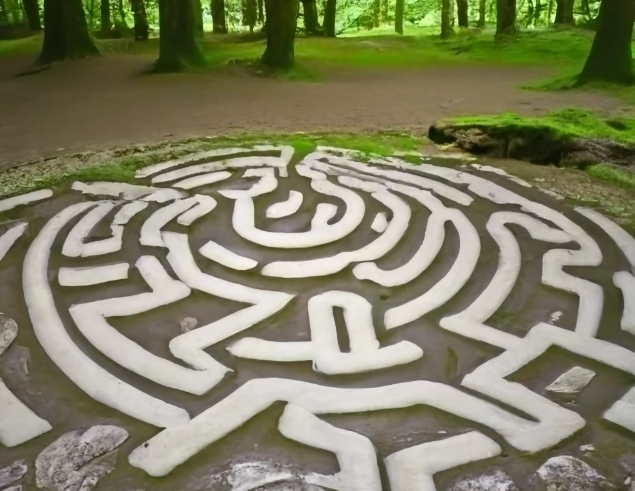
\includegraphics[scale=0.2]{./images/visuelAct1.png}

Aujourd'hui, le projet labyrinthe a commencé avec la visite d'André STEF, enseignant chercheur de l'université de Lorraine. Son expertise a été sollicitée pour initier la composante mathématique. Au-delà des chiffres et des équations, le projet labyrinthe révèle un lien intéressant avec la mythologie, où les labyrinthes ont souvent été des éléments intrigants dans des récits mythiques.

Mais, qu'est-ce qu'un labyrinthe, que ce soit dans la réalité ou dans les récits légendaires ? Les labyrinthes sont des structures complexes, déroutantes, et mystérieuses, souvent associées à des épreuves ou à des quêtes héroïques. Dans le cadre de ce projet, les élèves ont donc commencé par répondre à cette question. Ensuite, ils ont été confrontés à la tâche de création d'un algorithme de parcours sur papier.

L'approche choisie pour résoudre ce défi impliquait l'utilisation d'un algorithme avec un repérage relatif. Les élèves ont dû concevoir cet algorithme en se limitant à trois instructions simples : T pour "avancer d'une case tout droit", G pour "tourner d'un quart de tour sur la gauche et avancer d'une case", et D pour "tourner d'un quart de tour sur la droite et avancer d'une case". Ces instructions minimalistes, en apparence, ont nécessité une réflexion approfondie et une planification méticuleuse pour réussir à naviguer avec succès à travers le labyrinthe.

Après avoir élaboré leurs algorithmes, les élèves les ont mis à l'épreuve au laboratoire de mathématiques. C'est là qu'ils ont eu l'opportunité de valider ou d'invalider leurs solutions. Ce passage au laboratoire ajoute une dimension pratique cruciale au projet, permettant aux élèves de confronter leurs idées à la réalité du labyrinthe simulé.

Dans l'ensemble, le projet labyrinthe, initié par l'enseignant-chercheur André STEF, offre aux élèves une expérience mêlant mathématiques, et réflexion. C'est une aventure éducative qui pousse les limites de la créativité et de la résolution de problèmes, tout en se référant à la mythologie qu'ils étudieront en cours de français.
  
La suite du projet est à venir ...

Quelques photos et vidéos du jour
\subsubsection*{Deuxième séance - 1h}
% Proposition de labyrinthes

% Les élèves auront à concevoir des labyrinthes.

% L'activité se fera sous forme de DM navette classe/maison. Non noté !

% À l'issue, un labyrinthe sera choisi.
L'excitation régnait parmi les élèves lorsque le projet d'un labyrinthe dans la cour fut annoncé, certains sont même allés jusqu'à l'imaginer en 3D.
Imaginer un dédale mystérieux à explorer devint le défi central de la première séance. Chacun devrait mettre à contribution sa créativité
et ses compétences en conception pour donner vie à un labyrinthe unique.

À l'issue de cette première séance, les élèves se retrouveront avec des plans détaillés de leurs labyrinthes à réaliser en respectant certains contraintes.
Toutefois, avant de passer à l'étape suivante, une évaluation intermédiaire prendra la forme d'un DM navette. Cette évaluation servira
à identifier et corriger d'éventuels aspects problématiques de conception. Les enseignants offriront des retours constructifs, permettant
aux élèves d'affiner leur vision et d'améliorer la faisabilité de leur labyrinthe.

Vient ensuite la deuxième séance, où les élèves auront la tâche cruciale de sélectionner parmi leurs créations le labyrinthe qui sera
matérialisé dans la cour. Un processus démocratique guidera le choix, favorisant la participation et l'échange d'idées au sein de la classe.
Cela marquera le début de la transformation de leur vision imaginative en une réalité tangible.

Cependant, le défi ne s'arrête pas là. Les élèves seront confrontés à une question pratique : quelle longueur de mur sera nécessaire pour
donner forme à leur labyrinthe choisi ? Cette interrogation impliquera une exploration approfondie des notions de dénombrement et de proportionnalité.
Ils devront estimer la quantité de peinture requise, ce qui demandera une réflexion mathématique sur les dimensions du labyrinthe et
la longueur totale des murs.

Ainsi, ce projet transcende les limites de la créativité pour englober des compétences mathématiques essentielles. Le labyrinthe devient
une toile où se mêlent l'imagination artistique et les principes mathématiques concrets. À travers cette aventure, les élèves ne
construiront pas seulement un labyrinthe physique, mais aussi une compréhension approfondie des applications pratiques des mathématiques
dans le monde réel.

\subsection{Troisième temps - Réalisation du labyrinthe dans la cour}
Passer la surface au karsher au préalable.
Craie ? Peinture ? Adhesif ? 